\documentclass[a4paper, 12pt]{article}

%%% Работа с русским языком
\usepackage{cmap}					% поиск в PDF
\usepackage{mathtext} 				% русские буквы в формулах
\usepackage[T2A]{fontenc}			% кодировка
\usepackage[utf8]{inputenc}			% кодировка исходного текста
\usepackage[english, russian]{babel}	% локализация и переносы

\usepackage{color} 				 	% цветные буковки
\usepackage{listings}

\usepackage{caption}
\DeclareCaptionFont{white}{\color{white}}
%\DeclareCaptionFormat{listing}{\colorbox{gray}{\parbox{\textwidth}{#1#2#3}}}
\captionsetup[lstlisting]{format=listing,labelfont=white,textfont=white}

\usepackage{hyperref}
\usepackage{titlesec}
\usepackage{amsmath, amsfonts, amssymb, mathtools} 

%%% Поля страницы
\usepackage[top=20mm, bottom=20mm, left=30mm, right=15mm]{geometry}



%%% Вставка иллюстраций
\usepackage{graphicx}
\graphicspath{{img/}}

\usepackage{amsthm}

\theoremstyle{definition}
\newtheorem{defn}{Определение}[section]
\newtheorem*{rem}{Замечание}



%%% Format

% Математическое ожидание\
\newcommand{\Expect}{%
	\mathsf{M}}

\renewcommand{\Variance}{%
	\mathsf{D}}

% Математическое ожидание
\newcommand{\m}[1]{%
	\ensuremath{M\!#1}}

% Математическое ожидание X
\newcommand{\mx}{%
	\ensuremath{M\!X}}

\newcommand{\mxx}{%
	\ensuremath{M\!X^2}}

% Математическое ожидание Y
\newcommand{\my}{%
	\ensuremath{M\!Y}}

\newcommand{\myy}{%
	\ensuremath{M\!Y^2}}

% Дисперсия
\newcommand{\disp}[1]{%
	\ensuremath{D\!#1}}

% Дисперсия X
\newcommand{\dx}{%
	\ensuremath{D\!X}}

% Дисперсия Y
\newcommand{\dy}{%
	\ensuremath{D\!Y}}

% Следовательно
\newcommand{\Rarrow}{%
	\ensuremath{\;\Rightarrow\;}}

% Бесконечная последовательность 
\newcommand{\infseq}[3]{%
	\ensuremath{#1_#2, \dots, #1_#3, \dots}\ }

% Бесконечная последовательность X_1, ... X_n, ...
\newcommand{\infseqX}{%
	\infseq{X}{1}{n}}


%%% Код
\usepackage{listings,listingsutf8}

\lstset{
	frame = single,
	showstringspaces=false,
	basicstyle=\ttfamily\small,
	breaklines=true,
	xleftmargin=15pt, 
	framexleftmargin = 0pt,
	framextopmargin = 10pt,
	framexbottommargin = 10pt,
	literate={а}{{\selectfont\char224}}1
	{б}{{\selectfont\char225}}1
	{в}{{\selectfont\char226}}1
	{г}{{\selectfont\char227}}1
	{д}{{\selectfont\char228}}1
	{е}{{\selectfont\char229}}1
	{ё}{{\"e}}1
	{ж}{{\selectfont\char230}}1
	{з}{{\selectfont\char231}}1
	{и}{{\selectfont\char232}}1
	{й}{{\selectfont\char233}}1
	{к}{{\selectfont\char234}}1
	{л}{{\selectfont\char235}}1
	{м}{{\selectfont\char236}}1
	{н}{{\selectfont\char237}}1
	{о}{{\selectfont\char238}}1
	{п}{{\selectfont\char239}}1
	{р}{{\selectfont\char240}}1
	{с}{{\selectfont\char241}}1
	{т}{{\selectfont\char242}}1
	{у}{{\selectfont\char243}}1
	{ф}{{\selectfont\char244}}1
	{х}{{\selectfont\char245}}1
	{ц}{{\selectfont\char246}}1
	{ч}{{\selectfont\char247}}1
	{ш}{{\selectfont\char248}}1
	{щ}{{\selectfont\char249}}1
	{ъ}{{\selectfont\char250}}1
	{ы}{{\selectfont\char251}}1
	{ь}{{\selectfont\char252}}1
	{э}{{\selectfont\char253}}1
	{ю}{{\selectfont\char254}}1
	{я}{{\selectfont\char255}}1
	{А}{{\selectfont\char192}}1
	{Б}{{\selectfont\char193}}1
	{В}{{\selectfont\char194}}1
	{Г}{{\selectfont\char195}}1
	{Д}{{\selectfont\char196}}1
	{Е}{{\selectfont\char197}}1
	{Ё}{{\"E}}1
	{Ж}{{\selectfont\char198}}1
	{З}{{\selectfont\char199}}1
	{И}{{\selectfont\char200}}1
	{Й}{{\selectfont\char201}}1
	{К}{{\selectfont\char202}}1
	{Л}{{\selectfont\char203}}1
	{М}{{\selectfont\char204}}1
	{Н}{{\selectfont\char205}}1
	{О}{{\selectfont\char206}}1
	{П}{{\selectfont\char207}}1
	{Р}{{\selectfont\char208}}1
	{С}{{\selectfont\char209}}1
	{Т}{{\selectfont\char210}}1
	{У}{{\selectfont\char211}}1
	{Ф}{{\selectfont\char212}}1
	{Х}{{\selectfont\char213}}1
	{Ц}{{\selectfont\char214}}1
	{Ч}{{\selectfont\char215}}1
	{Ш}{{\selectfont\char216}}1
	{Щ}{{\selectfont\char217}}1
	{Ъ}{{\selectfont\char218}}1
	{Ы}{{\selectfont\char219}}1
	{Ь}{{\selectfont\char220}}1
	{Э}{{\selectfont\char221}}1
	{Ю}{{\selectfont\char222}}1
	{Я}{{\selectfont\char223}}1
}

\newcommand{\biglisting}[1]{%
	\lstinputlisting[numbers=left]{#1}%
}
\begin{document}

\thispagestyle{empty}

\begin{center}
	\Large
	Московский государственный технический университет имени~Н.\,Э.\,Баумана
\end{center}

\hfill\begin{minipage}{0.77\textwidth}
	{\large
		\noindent
		Факультет: Фундаментальные науки\\[2mm]
		\noindent
		Кафедра:  Математическое моделирование\\[2mm]
		\noindent
		Дисциплина: Математическая статистика 
		\vspace{1.5cm}}
\end{minipage}
\vfill

\begin{center}
	\Large
	\textbf{Лабораторная работа №3 \\}
	\textbf{Метод наименьших квадратов} \\
\end{center}
\vfill

\hfill\begin{minipage}{0.35\textwidth}\textsl{}
	Выполнила: Покасова А.И.\\
	Группа:ИУ7-61 \\
	Вариант: 16
\end{minipage}
\vfill

\begin{center}
	Москва, \the\year\space г.
\end{center}

\newpage
\section{Постановка задачи}

\paragraph{Цель работы:}аппроксимация неизвестной зависимости параболой.

\paragraph{Содержание работы:}
\begin{enumerate}
	\item Для выборки $(y_i, t_i)$, $i = \overline{1; n}$, реализовать в виде программы на ЭВМ:
	\begin{enumerate}
		\item вычисление МНК-оценки $\vec\theta = (\theta_0, \theta_1, \theta_2)$ параметров модели $y = \theta_0 + \theta_1 t + \theta_2 t^2$;
		\item вычисление среднеквадратичного отклонения $$\Delta = \sqrt{\sum_{i=1}^{n}\left(y_i - y(t_i)\right)^2}$$ полученной модели от результатов наблюдений;
		\item построение на одном графике системы точек $(y_i, t_i)$, $i = \overline{1; n}$, и графика функции $y = y(t)$, $t \in \left[t_{(1)}; t_{(n)}\right]$ (для полученной оценки $\vec\theta$\,).
	\end{enumerate}
	\item провести необходимые вычисления и построить соответствующие графики для выборки из индивидуального варианта.
\end{enumerate}

\paragraph{Содержание отчёта:}
\begin{enumerate}
	\item постановка задачи аппроксимации неизвестной зависимости по результатам наблюдений;
	\item понятие МНК-оценки параметров линейной модели;
	\item формулы для вычисления МНК-оценки в рассматриваемом случае;
	\item текст программы;
	\item результаты расчетов и графики для выборки из индивидуального варианта.
\end{enumerate}

\pagebreak
\section{Отчёт}

\section{Теоретическая часть}

\subsection{Постановка задачи аппроксимации неизвестной зависимости по результатам наблюдений}

Пусть Y – случайная величина, $X_1, \dots, X_s$ – детерминированные величины. Если изменение значений $X_1, \dots, X_s$ влияет на значения случайной величины Y, то говорят, что Y стохастически зависит от $X_1, \dots, X_s$. Задача регрессионного анализа – задача, связанная с установлением аналитических зависимостей между случайной величиной Y и детерминированными величинами $X_1, \dots, X_s$, носящими количественный характер. 
В регрессионном анализе используется модель черного ящика, как наиболее общая модель, ассоциируемая с понятием отображения. На вход поступает вектор $X_1, \dots, X_s$, который посредством некоторого отображения $\Phi$ и случайных возмущений $\varepsilon_1, \dots, \varepsilon_n$ преобразуется в вектор $Y_1, \dots, Y_m$.

\subsection{Понятие МНК-оценки параметров линейной модели}

Предположим, что в нашем распоряжении имеются результаты $n$ наблюдений:
\begin{equation}
\begin{cases}
y_1 = \Phi(x_1) + \varepsilon_1 \\
\qquad\cdots                    \\
y_n = \Phi(x_n) + \varepsilon_n \\
\end{cases}, \quad \text{где}
\end{equation}
\begin{itemize}
	\item $y_1, \dots, y_n$ --- $n$ реализаций $Y$;
	\item $\varepsilon_1, \dots, \varepsilon_n$ --- $n$ реализаций $\varepsilon$;
	\item $x_1, \dots, x_n$ -- известные значения.
\end{itemize}
Требуется на основе этих данных подобрать функцию $\widehat{\Phi}$ так, чтобы она наилучшим образом аппроксимировала неизвестную функцию $\Phi$.


Часто в качестве функции $\widehat{\Phi}(x)$ выбирают функцию следующего вида:
\begin{equation}
\widehat{\Phi}(x) = \theta_1 \psi_1(x) + \dots + \theta_p \psi_p(x), \quad \text{где}
\end{equation}
\begin{itemize}
	\item $\psi_1, \dots, \psi_p$ --- базисные функции.
\end{itemize}
Параметры $\theta_1, \dots, \theta_p$ подбирают так, чтобы $\widehat{\Phi}(x)$ наилучшим образом аппроксимировала $\Phi(x)$.

С учётом предположения о виде функции $\widehat{\Phi}$ результаты наблюдений можно записать в виде:
\begin{equation}
y_i = \theta_1 \psi_1(x_i) + \dots + \theta_p \psi_p(x_i) + \varepsilon_i, \quad i = \overline{1; n}\,.
\end{equation}
В матричном виде:
\begin{equation}
\vec{y} = \Psi \vec{\theta} + \vec{\varepsilon}, \quad \text{где}
\end{equation}
\begin{align*}
& \vec{y} = \begin{pmatrix} 
y_1    \\ 
y_2    \\ 
\vdots \\ 
y_n 
\end{pmatrix},
& \Psi &= \begin{pmatrix}
\psi_1(x_1) & \psi_2(x_1) & \cdots & \psi_p(x_1) \\
\psi_1(x_2) & \psi_2(x_2) & \cdots & \psi_p(x_2) \\
\vdots      & \vdots      & \ddots & \vdots      \\
\psi_1(x_n) & \psi_2(x_n) & \cdots & \psi_p(x_n)
\end{pmatrix},
& \vec{\theta} &= \begin{pmatrix}
\theta_1 \\
\theta_2 \\ 
\vdots   \\ 
\theta_p
\end{pmatrix},
& \vec{\varepsilon} = \begin{pmatrix} 
\varepsilon_1 \\
\varepsilon_2 \\ 
\vdots        \\ 
\varepsilon_n
\end{pmatrix}.
\end{align*} 
Задача заключается в подборе $\vec{\theta}$.

Будем предполагать, что:
\begin{enumerate}
	\item $M\varepsilon = 0$, т.\,е. систематические ошибки отсутствуют;
	\item $\varepsilon \sim N(0, \sigma^2)$.
\end{enumerate}

\begin{defn}
	Оценка $\hat{\vec{\theta}}$ вектора $\vec{\theta}$ называется \emph{оценкой}, полученной по \emph{методу наименьших квадратов (МНК-оценкой)}, если $\vec{\theta}$ доставляет минимальное значение функции $S(\vec{\theta}) = \|y - \Psi \vec{\theta}\|^2$.
\end{defn}


\subsection{Формулы для вычисления МНК-оценки в рассматриваемом случае}

В рассматриваемом случае МНК-оценка вектора $\vec{\theta}$ имеет вид:
\begin{equation}
\hat{\vec{\theta}} = (\Psi^T \Psi)^{-1} \cdot \Psi^T \vec{y}\,, \quad \text{где}
\end{equation}
\begin{itemize}
	\item $\mathsf{rg}(\Psi) = p$ --- числу столбцов.
\end{itemize}
причём так как $y = \theta_0 + \theta_1 t + \theta_2 t^2$, то
\begin{equation}
\Psi = \begin{pmatrix}
1      & t_1    & t_1^2  \\
1      & t_2    & t_2^2  \\
\vdots & \vdots & \vdots \\
1      & t_n    & t_n^2
\end{pmatrix}.
\end{equation}


Среднеквадратичное отклонение полученной модели от результатов наблюдений будем вычислять как
\begin{equation}
\Delta = \sqrt{\sum_{i=1}^{n}\left(y_i - y(t_i)\right)^2}, где
\end{equation}

\begin{itemize}
	\item $y_i$ -- результат наблюдения
	\item $y(t_i)$ -- результат аппроксимации
\end{itemize}

\section{Текст программы}

\lstinputlisting{lab3.m}

\section{График}

График исходной выборки и полученной модели

\begin{figure}[h]
	\centering
	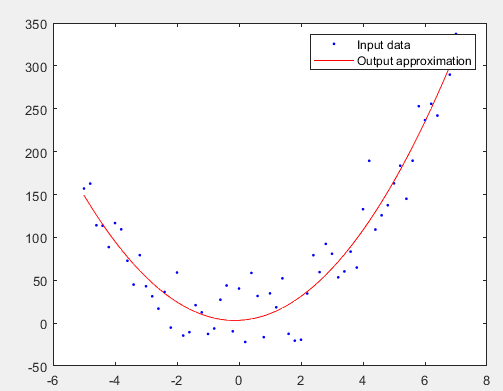
\includegraphics[scale=1.0]{1.png}
\end{figure}

\end{document}